\documentclass[11pt]{article}

\usepackage{amsfonts}
\usepackage{amsmath}
\usepackage{graphicx}
\usepackage{fullpage}
\usepackage[utf8]{inputenc}
\usepackage[czech]{babel}

\usepackage{hyperref}

\def\code#1{\texttt{#1}}
\author{Vojtěch Pröschl}
\title{Statistická Práce \\ \large Robotický Vysavač}


\begin{document}
\maketitle


\section{Prostředí experimentu}
\paragraph{Stručné shrnutí:} Máme robota, který se v pokoji pohybuje tak, že jde rovně, dokud nenarazí do zdi. Pokud narazí do zdi, otočí se o náhodný úhel a pokračuje rovně. Ve zbytku této sekce je detailněji popsán model světa, ve kterém se experiment odehrává, a konkrétní „mechanismus“ fungování robota.

\subsection{Pokoj}
\paragraph{Geometrie:} Podlaha pokoje je popsána polygonem $A$, překážky jsou popsány polygony $B,C$ a $D$. Body, které leží uvnitř polygonu $A$ a zároveň neleží uvnitř polygonů $B,C$ nebo $D$ reprezentují plochu, kterou má robot uklidit.

\begin{center}
	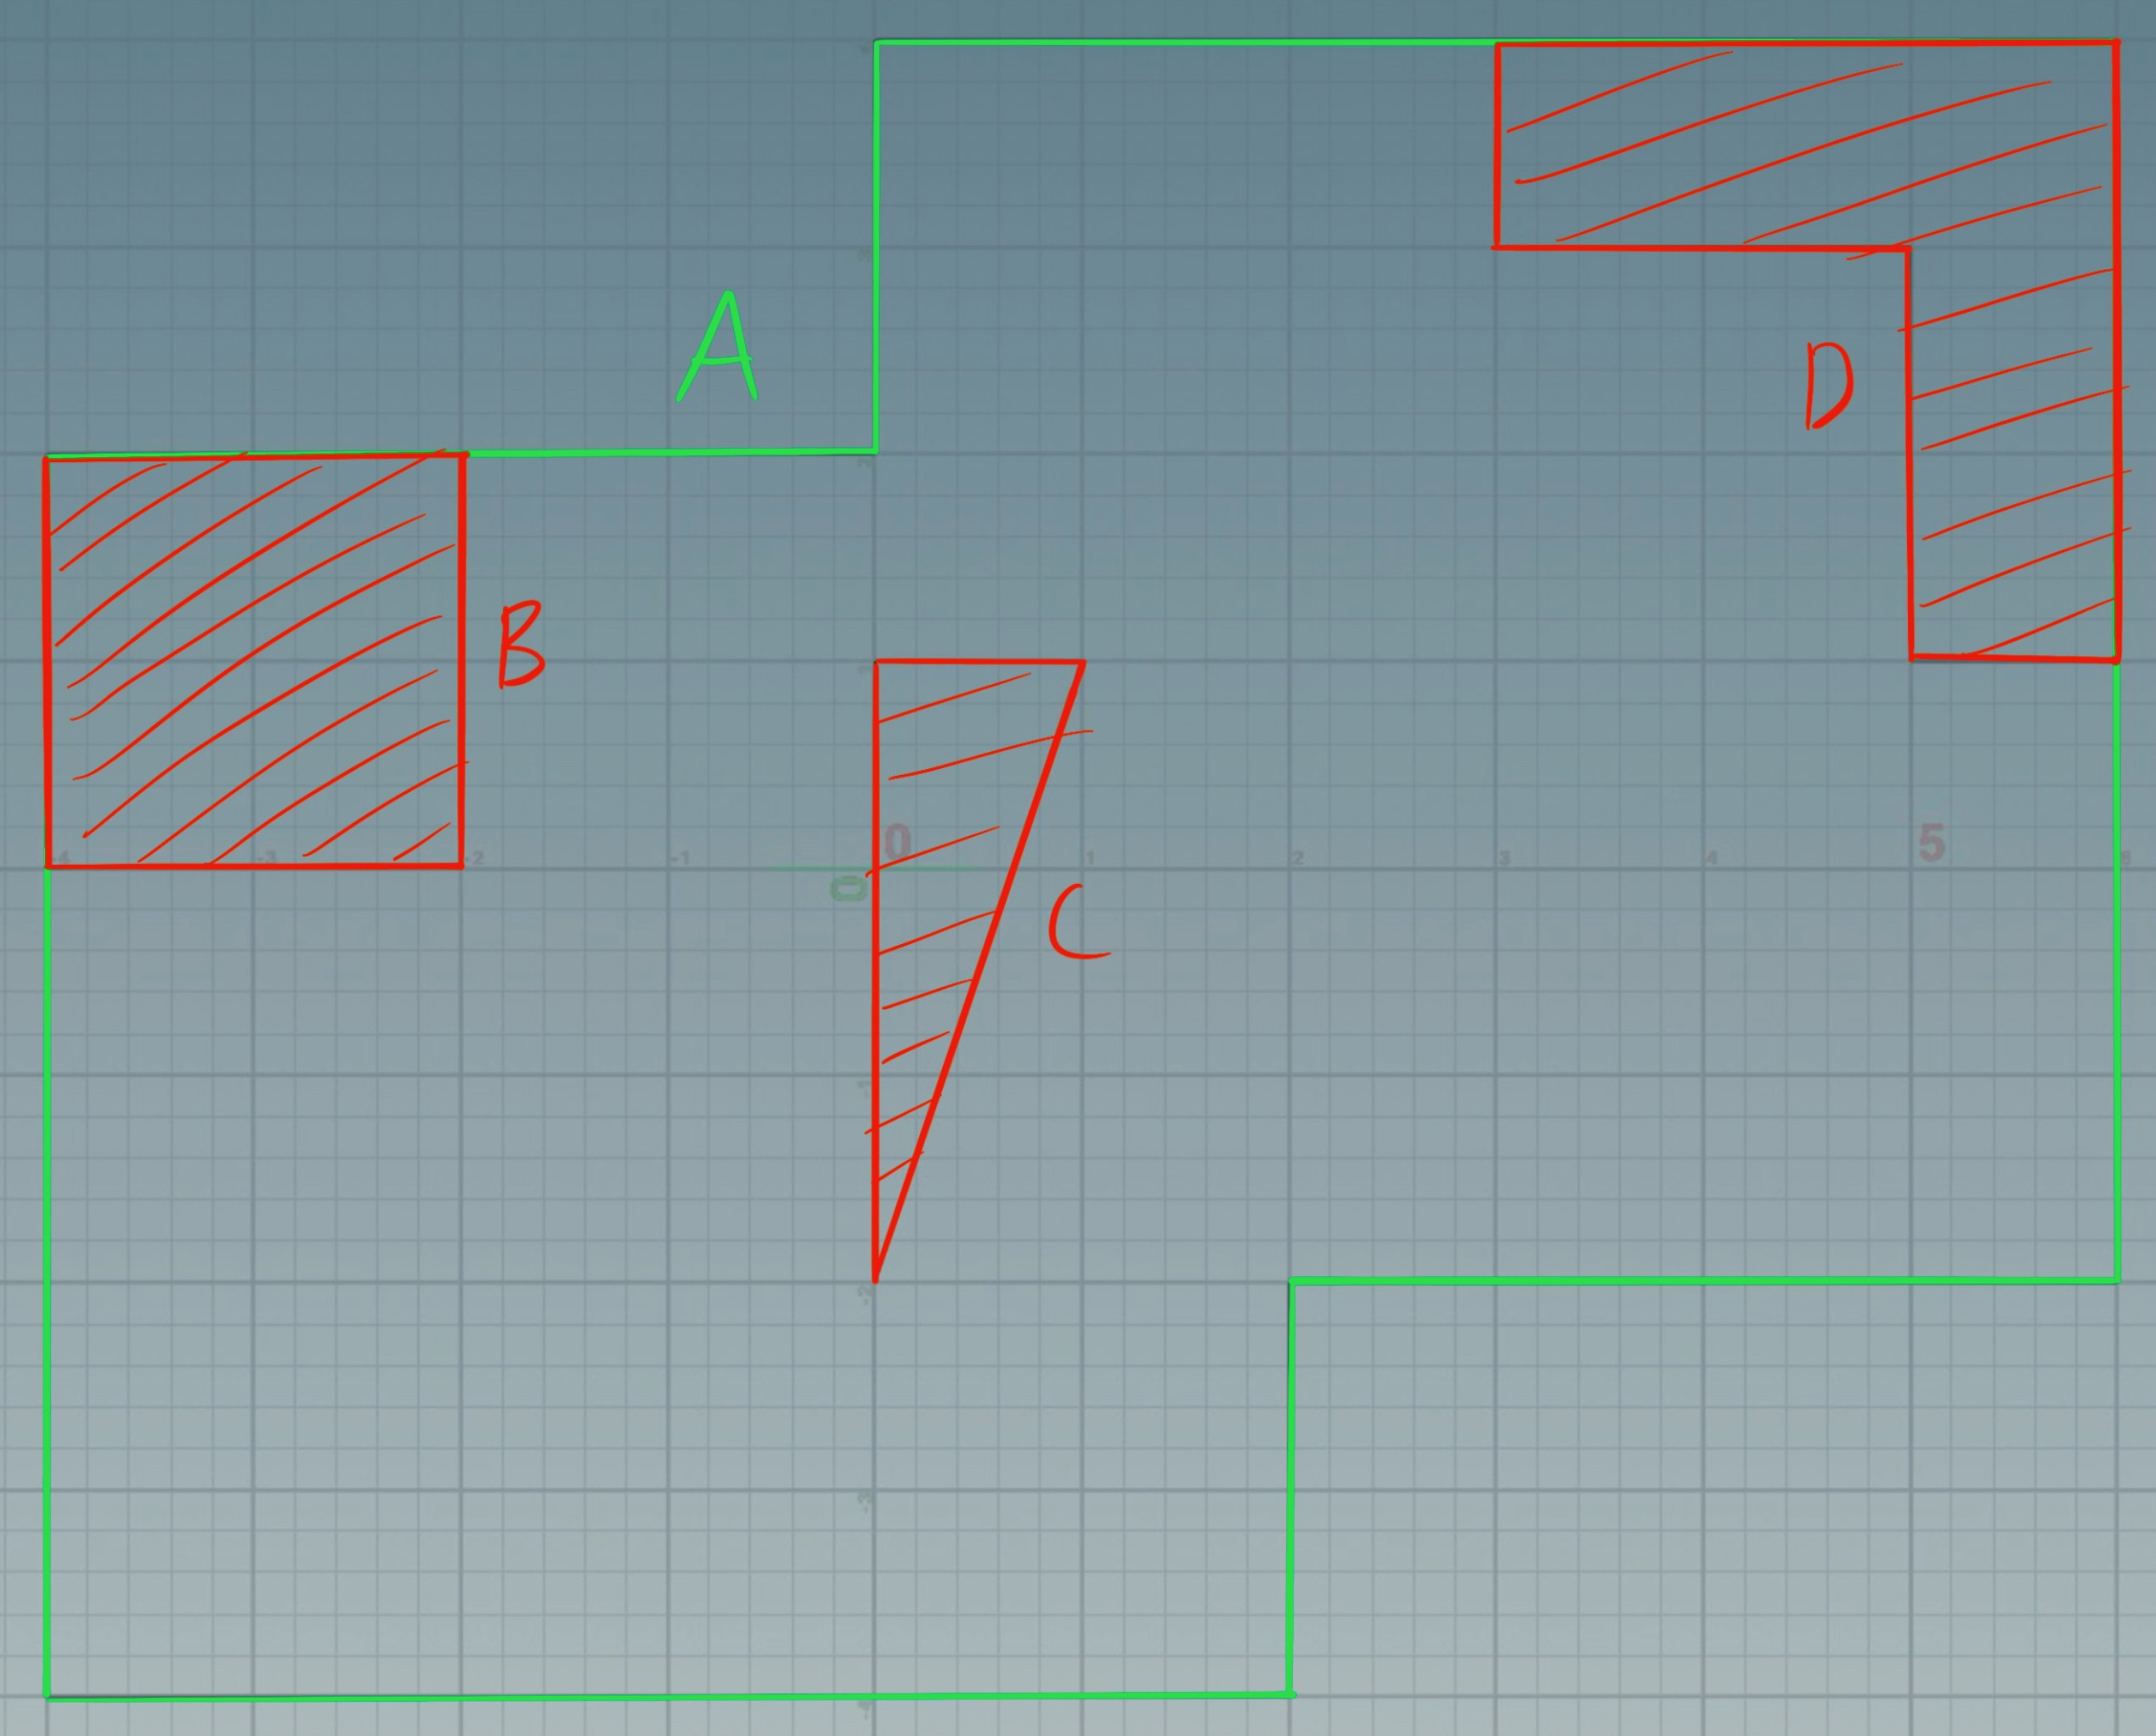
\includegraphics[scale=0.27]{Images/RoomGeometry.jpeg}
\end{center}


\paragraph{Úklidové body:} Na ploše podlahy, která není zablokována žádnou z překážek, jsem uniformně náhodně vygeneroval $20$ tisíc bodů, které budou reprezentovat nepořádek v pokoji.

\begin{center}
	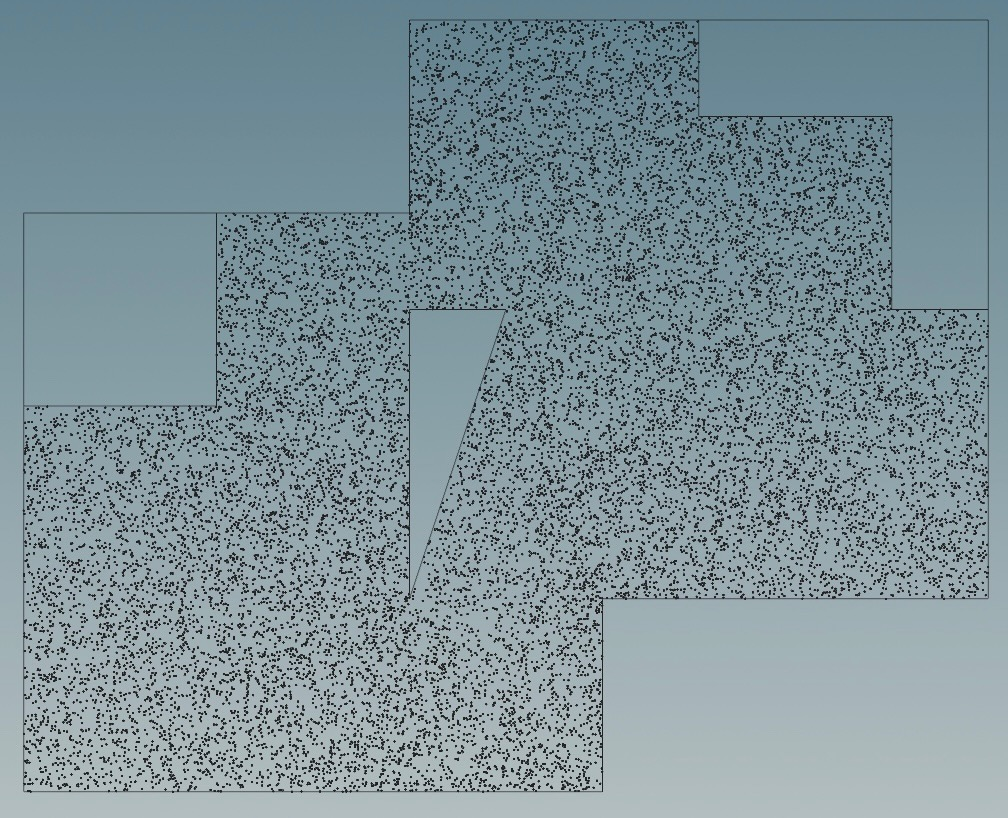
\includegraphics[scale=0.37]{Images/RoomDebris.jpeg}
\end{center}

\subsection{Robot}
Robot je z geometrického pohledu kruh v prostoru, který je schopen uklidit body, které do něj v daný moment náleží. Robot má přiřazenou určitou orientaci. Je schopen se pohybovat rovně ve směru této orientace a otáčet se, aby změnil svou orientaci.
\paragraph{Radius:}
$$
r:=0.15
$$
\paragraph{Startovni pozice:}
$$
S_P=(-2,-2)
$$
\paragraph{Startovni orientace:}
$$
S_o=0
$$
Poznámka: toto reprezentuje směr robota  $(\cos(0),\sin(0))$

\paragraph{Rychlost pohybu:}
$$
v:=0.3\; \left[\frac{m}{s}\right]
$$
\paragraph{Rychlost otáčení:}
$$
\omega := \frac{\pi}{5} \;\left[\frac{\mathrm{rad}}{s} \right]
$$

\subsection{Dostupné instrukce:}
\paragraph{Move forward:} Robot půjde rovně, dokud nenarazí do zdi. Doba trvání této instrukce se počítá jako 
$$
t_m=\frac{d_e(P_0,P_1)}{v}
$$
kde $P_0$ je pozice, na které robot začal, a $P_1$ je pozice, na které robot narazil do zdi.

\paragraph{Rotate by $\alpha$:} Robot se otočí o úhel $\alpha$ kolem své osy. Doba trváni této instrukce je
$$
t_r=\frac{\alpha}{\omega}
$$

\subsection{Algoritmus robota}
Posloupnost instrukcí robota je funkce $I:\mathbb{N}\to \mathrm{Instructions}$

$$
I(k)=
\begin{cases}
\text{Move forward} & \iff k \;\%\;2=0\\
\text{Rotate by }\alpha(k) & \iff k\;\%\;2=1
\end{cases}
$$
Kde $\alpha:\mathbb{N}\to [-\pi,\pi]$ je konkrétní pozorování posloupnosti uniformně rozdělených, nezávislých náhodných veličin na výše uvedeném intervalu. 


\subsection{Proces uklidu}
Pokud je v nějakém okamžiku vzdálenost středu robota od nějakého úklidového bodu menší než jeho poloměr, tento bod se označí za uklizený. Procento uklizené plochy můžeme aproximovat pomocí úklidových bodů jako:
$$
\frac{\#\text{Uklizených}}{\#\text{Úklidových bodu}} \cdot 100
$$
Aby se experiment dal realizovat v rozumném čase, přepočítávám počet uklizených bodů vždy po dokončení instrukce.

\begin{center}
	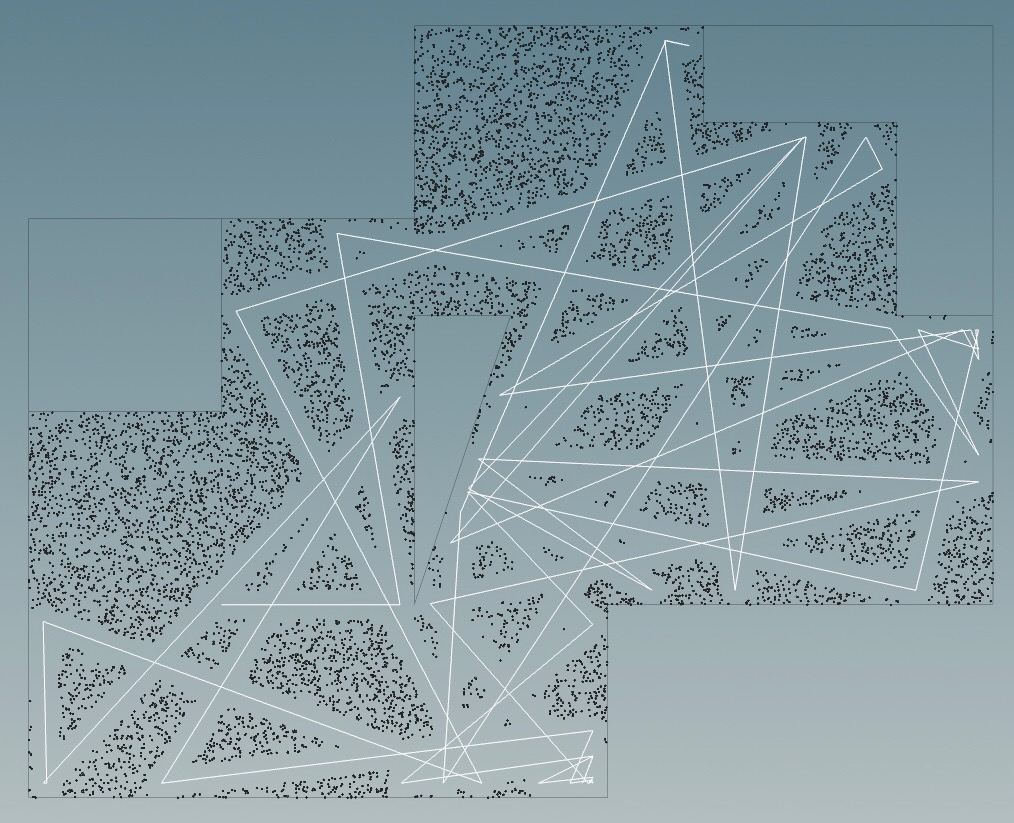
\includegraphics[scale=0.35]{Images/CleaningPath.jpeg}
\end{center}

\section{Experiment}
Cílem experimentu je nasbírat data o chování robota při úklidu modelového prostředí.
\subsection{Jedna iterace}
Iteraci si rozdělíme na jednotlivé instrukce a budeme sbírat data o stavu úklidu po vykonání k-té instrukce. Celkem v jedné iteraci provedeme $5000$ instrukcí. Data, která budeme sbírat, jsou následující:
\begin{itemize}
	\item $T_I$ - Jak dlouho robotovi trvala k-tá instrukce?
	\item $T_C$ - Jak dlouho robotovi celkem trvalo vykonat instrukce 0 až k?
	\item $C_I$ - Kolik dosud neuklizených bodů robot při vykonávání k-té instrukce uklidil?
	\item $C_C$ - Kolik bodů je po vykonání k-té instrukce celkem uklizeno?
	\item $P$ - Kolik procent bodů je po vykonání k-té instrukce uklizeno?
\end{itemize}

\subsection{Opakované iterace}
Provedeme $2\cdot 500$ iterací našeho experimentu. V každé iteraci pro generování náhodných čísel pro rotace použijeme jiný seed. Výsledné data jsem rozdělil do dvou skupin, prvních 500 běhů jsem uložil do složky \code{/Data/DataSet1} a posledních 500 běhů jsem uložil do složky \code{/Data/DataSet2}. V následující sekci provedu explorační analýzu dat z první množiny, pomocí které zformuluju hypotézu. Tuto hypotézu pak budu testovat na druhé množině dat.

\subsection{Jak jsem prováděl simulace?} Simulace jsem prováděl v softwaru SideFX Houdini, v repozitáři je uložený soubor s experimentem \code{/Houdini/main.hiplc}. Houdini je program na procedurální generování geometrie a simulace a má solidní sadu nástrojů na výpočetní geometrii, pomocí čehož jsem vytvořil simulátor. Nekomerční verze softwaru se dá zdarma stáhnout na \href{http://www.sidefx.com}{stránce SideFX}.

\section{Explorační analýza dat - Experiment 1}
Výpočty z této částí jsou popsány ve zdrojáku \code{ExperimentExploration.py}. Cílem je prozkoumat chování robota během jednoho běhu. Běh, který zde analyzuji je \code{/Data/DataSet1/Experiment1.csv}.

\subsection{O jednotlivých instrukcích}
Pojďme se nejprve podívat na to, jak dlouho trvaly jednotlivé instrukce.
\begin{itemize}
	\item Nejkratší instrukce $\approx 1.98\cdot 10^{-7} \;[s]$
	\item Nejdelší instrukce $\approx 34.5\;[s]$
	\item Průměrná instrukce $\approx 3.9 \;[s]$
	\item Průměrná \code{Move} instrukce $\approx 5.3 \;[s]$
	\item Průměrná \code{Rotate} instrukce $\approx 2.49 \;[s]$
\end{itemize}
Protože se robot otáčí vždy o úhel $\alpha\in [-\pi,\pi]$, který si vybírá uniformě náhodně, můžeme odvodit, že průměrné otočení trvá $(\pi/2)/(\pi/5)=5/2$ sekund - tohle poměrně dobře odpovídá pozorovaným datům.
Z toho rovněž pomocí rychlosti pohybu $v$ můžeme odvodit průměrnou vzdálenost, kterou robot při pohybové instrukcí urazí jako $5.3\cdot v=1.674$

\subsection{Rozdělení trvání instrukcí}
\begin{center}
	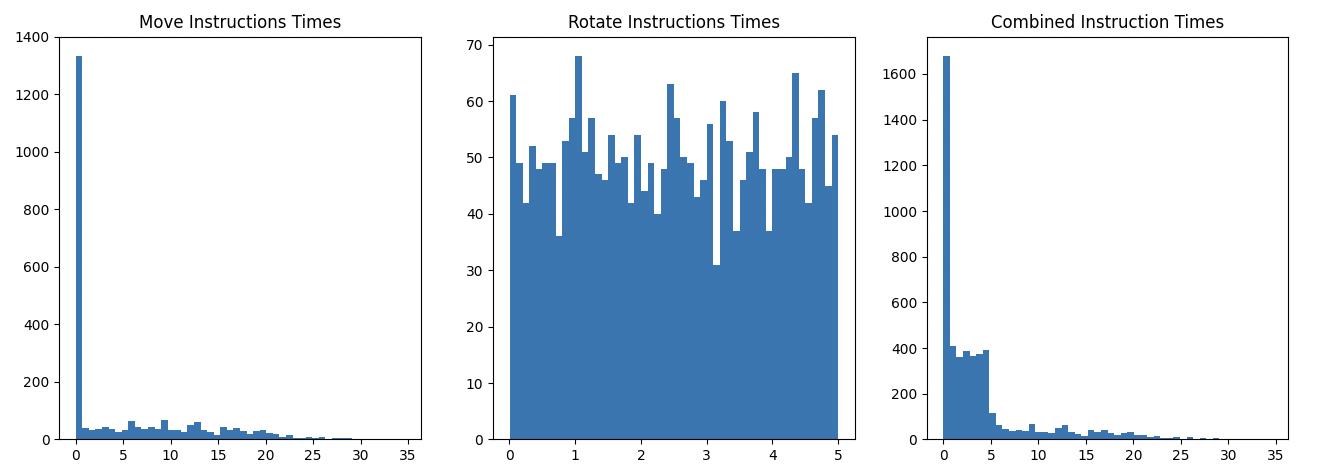
\includegraphics[scale=0.35]{Images/Section32_2.png}
\end{center}
Z rozdělení instrukcí můžeme vypozorovat pár zajimavých vlastností robota
\paragraph{Opakované nárazy do zdi:} V momentě, kdy robot narazí do zdi, se často stává, že po otočení robot neujde moc velkou vzdálenost a opět narazí do té samé zdi (spike v prvním histogramu). Tohle nám ale z hlediska doby úklidu moc nevadí, protože takové instrukce jsou velmi rychlé.

\paragraph{Otáčení zabírá hodně času:} Problém ale nastává v tom, že po nárazu do zdi, se robot opět otočí o náhodný úhel, což průměrně trvá 2.5s. Ke každé zanedbatelné instrukci pohybu, při které robot narazí do zdi hned po otočení, si tedy musíme přičíst čas, jaký trvalo samotné otočení. Algoritmus by se tedy dal dost zrychlit, kdybychom zamezili opakovaným nárazům do zdi (nebo chytřeji volili rotaci po opakovaném nárazu)

\paragraph{Rozdělení času:} Rozdělení doby trvání instrukcí je dost složité a pravděpodobně by se dalo modelovat kombinací několika známých rozdělení. V tomhle projektu se tímhle směrem nevydáme, a raději budeme měřit dobu celkového úklidu.
\subsection{O celkovém průběhu}
Robotovi v experimentu 1 trvalo vykonat $5000$ instrukci priblizne $19518$ sekund a uklidil pri tom priblizne $97.79\%$ plochy pokoje. 
\begin{center}
	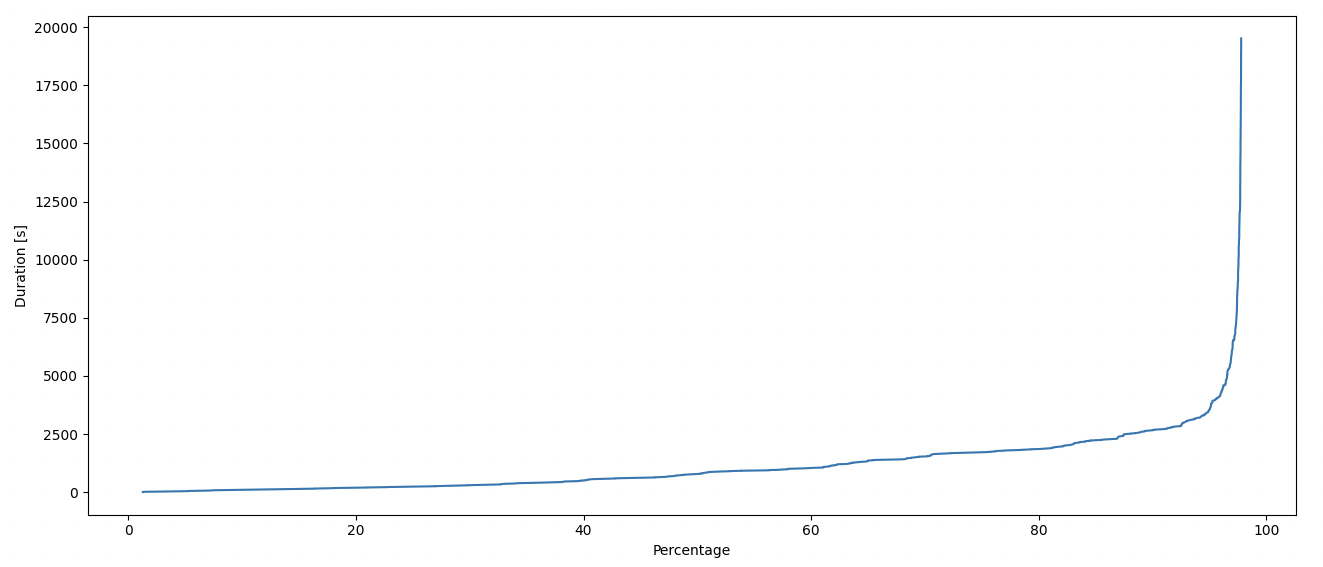
\includegraphics[scale=0.34]{Images/DurationPercentageSingle.png}
\end{center}
Z tohoto grafu můžeme vyčíst, že zřejmě časová náročnost pro uklizení dalšího procenta po překročení hranice přibližně 90ti procent opravdu strmě roste. Z praktického pohledu by nám mohlo stačit, aby robot uklidil právě $90\%$ plochy pokoje. V další části tedy prozkoumáme, jak vypadá rozdělení časů, kdy robot překročil hranici $90\%$.

%
%\subsection{Teoretické maximum}


\section{Explorační analýza dat - Dataset 1}
Výpočty z této částí jsou popsány ve zdrojáku \code{DataSetExploration.py}
\subsection{O celkovém průběhu}
Podobně jako v části s jedním experimentem, podívejme se na to, jakým způsobem vypadá chování mnoha experimentů - v tomto případě celého datasetu 1. Pro sjednocení dat jsem na základě výsledků experimentů provedl lineární interpolaci dat a každý experiment jsem nasamploval na interval $[5,97]$ procent. Tohle do dat přivádí určitou nepřesnost, vzhledem k tomu, že ale robot typicky v jedné instrukci neuklidí moc velkou plochu, je to přijatelné.
\begin{center}
	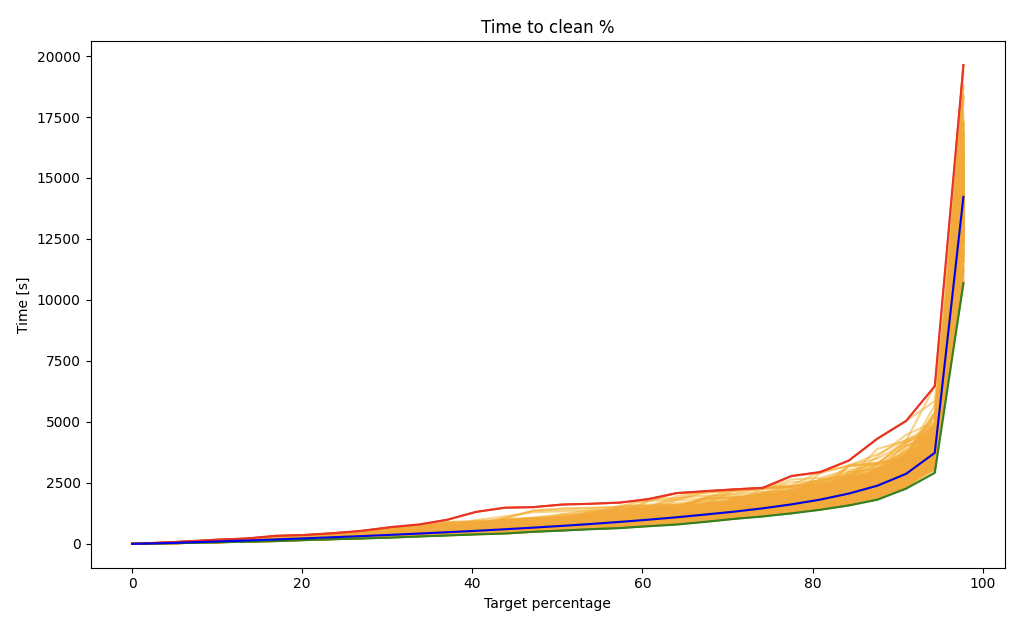
\includegraphics[scale=0.4]{Images/PercentageDS1.png}
\end{center}
Na teto ilustraci modrá červená křivka je vrchní hranice doby trvání pro určité procento uklizené plochy, modrá je střední hodnota a zelená křivka je minimální doba trvání. Z těchto dat je patrné, že rozptyl doby pro úklid určité plochy roste podobně jako čas. Nicméně v $90\%$ je stále jak střední hodnota doby úklidu, tak rozptyl této doby poměrně přijatelný, pojďme se na to teď podívat jako na rozdělení.
\subsection{Jak dlouho trvá uklidit $90\%$ plochy?}
Pojďme se nejprve podívat na histogram o tomto údaji pro všech 500 úklidů z datasetu1.
\begin{center}
	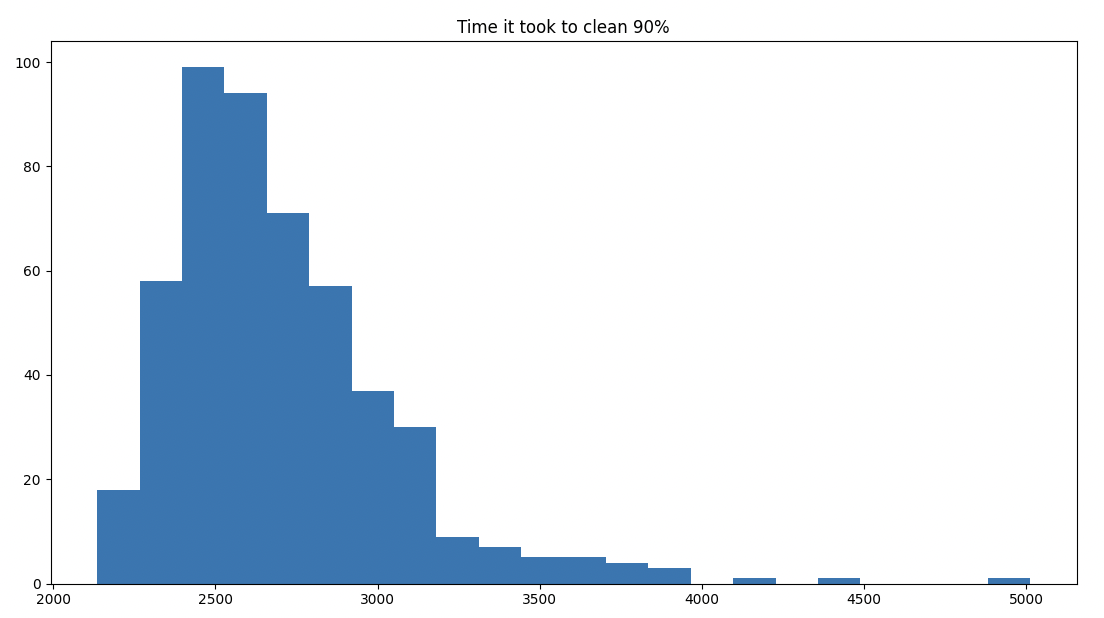
\includegraphics[scale=0.4]{Images/HistogramDataset.png}
\end{center}
Z histogramu se může zdát, že jsou doby normálně rozdělené, problém je ale v tom, že je pro vysavač nemožné uklidit dané procento rychleji, než je nějaký minimální čas úrčený jeho parametry a geometrii pokoje. Z moje pohledu tohle poměrně dobře odpovídá \href{https://en.wikipedia.org/wiki/Log-normal_distribution}{log-normálnímu rozdělení}.
\subsection{ECDF a fitting parametrů}
Provedu fitting parametrů log-normálního rozdělení na základě dat z datasetu 1.
\begin{center}
	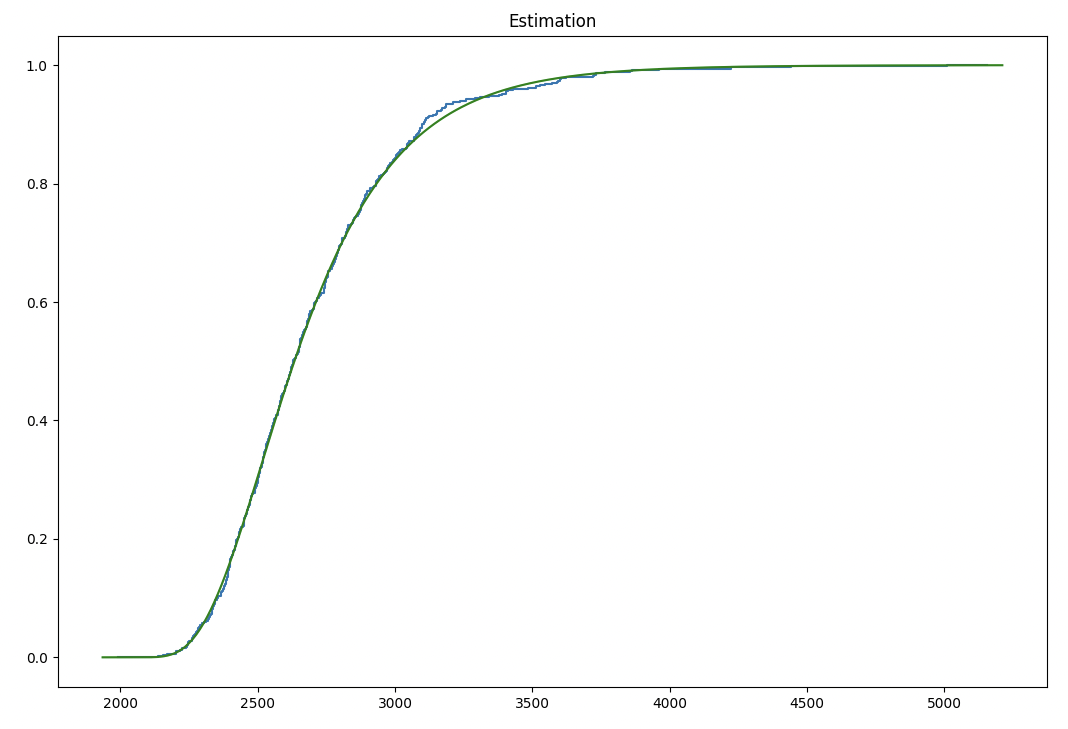
\includegraphics[scale=0.3]{Images/EstimationCDF.png}
\end{center}
Zde modrá křivka reprezentuje ECDF a zelená křivka reprezentuje log-normální rozdělení s výpočetně odhadnutými parametry. Tyto parametry pro nás budou tvořit hypotézu o distribuci této náhodné veličiny.
\subsection{Hypotéza}
Nulová hypotéza pro nás bude následující. Rozdělení časů pro úklid právě $90\%$ plochy našeho pokoje se řídí log-normálním rozdělením s následujícími parametry
\begin{itemize}
	\item $\mathrm{Shape} = 0.4489822310415079$
	\item $\mathrm{Loc} = 1982.106368481833$
	\item $\mathrm{Scale}= 651.5013077189651$
\end{itemize}

\section{Testování hypotézy}
Výpočty z této částí jsou popsány ve zdrojáku \code{HypothesisTest.py}
\subsection{Metoda testování}
Pro testování hypotézu použijeme dataset2, který nebyl použit při odvozování parametrů našeho rozdělení, takže nedochází k over-fittingu.
\begin{center}
	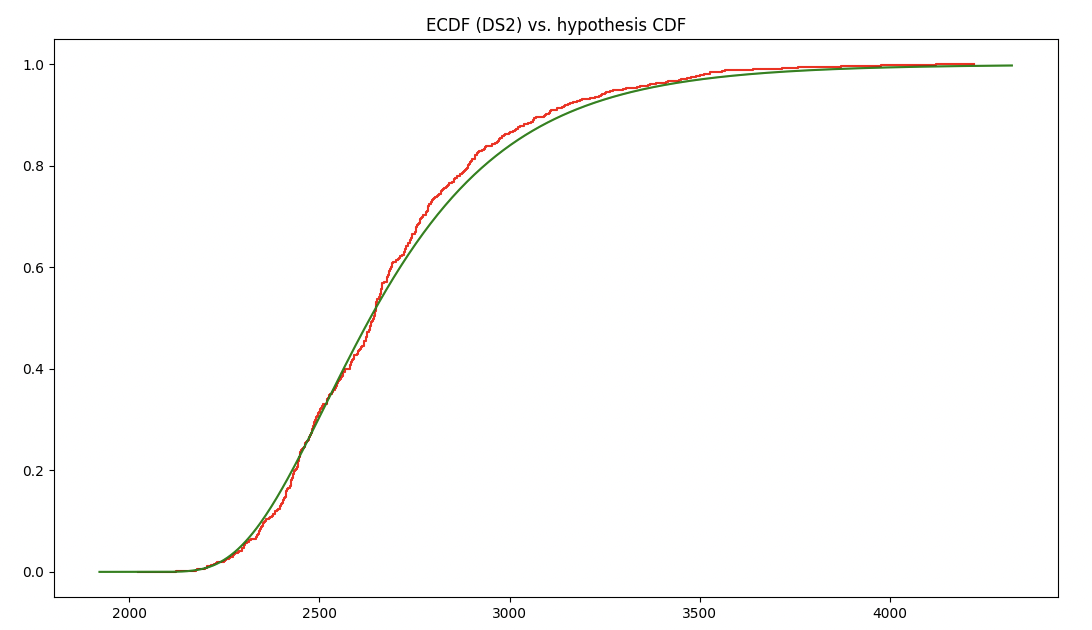
\includegraphics[scale=0.4]{Images/ECDFDS2.png}
\end{center}
ECDF v tomto případě neodpovídá odhadnuté CDF tak perfektně jako v případě ECDF založené na datasetu1, stále to ale vypadá jako velmi dobrý odhad. Pro testování použijeme hladinu významnosti $\alpha=0.05$ a pro testování použijeme Kolmogorov-Smirnov test.
\subsection{Kolmogorov-Smirnov test}
KS test pro data z datasetu2 testovaná vůči CDF z naší hypotézy dává $\mathrm{p-value}=0.31606614339733397$, což je výrazně víc než naše hladina významnosti a nemáme tedy důvod nulovou hypotézu zamítat.

\section{Další hypotézy}
Výpočty z této částí jsou popsány ve zdrojáku \code{HypothesisTestMultiple.py}
\subsection{Jak je to pro jiné procenta?}
Náš výsledek se zdá docela přesvědčivý pro $90\%$, jak je to ale s rozdělením pro jiné cílové procenta? Provedu analogický odhad parametrů, log-normálního rozdělení pro různé cílové procenta, konkrétně $10, 20, 30, 40, 50, 60, 70, 80$ procent.
\subsection{Hypotézy}
Formátování: shape loc scale
\begin{itemize}
	\item $10\%:0.3052524424624377\;\;45.14648389155834\;\;53.94814502257164$
	\item $20\%:0.34367812078306403\;\;116.65825225799732\;\;103.58640645864718$
	\item $30\%:0.4535664109752615\;\;228.77286605431138\;\;125.40188821453374$
	\item $40\%:0.5331781106784712\;\;364.99659944511353\;\;144.0250888637354$
	\item $50\%:0.5160261024537106\;\;503.787822221032\;\;196.87174563091259$
	\item $60\%:0.4963277813879759\;\;675.5620313021955\;\;264.05164841303406$
	\item $70\%:0.5362315708451335\;\;948.9188838985673\;\;299.4146138141141$
	\item $80\%:0.44030798855585473\;\;1275.8121167299041\;\;440.65809345802916$
\end{itemize}
\subsection{Testy hypotéz}
KS testy pro našich 8 hypotéz dopadly následovně
\begin{itemize}
	\item $10\%:\mathrm{p-value}=0.28871940536068397$
	\item $20\%:\mathrm{p-value}=0.9845237449337881$
	\item $30\%:\mathrm{p-value}=0.22367017712890935$
	\item $40\%:\mathrm{p-value}=0.2598277492024311$
	\item $50\%:\mathrm{p-value}=0.23905445718213625$
	\item $60\%:\mathrm{p-value}=0.10273493786799737$
	\item $70\%:\mathrm{p-value}=0.1284398556680877$
	\item $80\%:\mathrm{p-value}=0.5941981637483178$
\end{itemize}
Pro zvolenou hranici významnosti $\alpha=0.05$, tedy všechny naše hypotézy prošly a nemáme je důvod zamítat. Zajímavé je, že některých případech se p hodnoty poměrně výrazně liší a mohlo být zajímavé prozkoumat proč tomu tak je. Každopádně tahle otázka je už nad rámec této práce.
\end{document}
